%%%%%%%%%%%%%%%%%%%%%%%%%%%%
% Prototype Implementation %
%%%%%%%%%%%%%%%%%%%%%%%%%%%%

\chapter{Prototyp-Implementierung}
\label{chapter:prototype}

\section{Übersicht}

% Anforderungen an den Prototypen?

% Wahl der Technologie
% Das Layout-Framework von Sonja Maier konnte nicht als Grundlage verwendet werden, da nicht veröffentlicht
% Dunnart Biblitheken

% - eine neu entwickelte App
% - native Mac OS X App
% - Standardbibliotheken: Cocoa, Quartz
% - genutzte API's
% - Objective-C
% - keine weiteren Abhängigkeiten

% kurze Beschreibung des Prototypen
% Screenshot, Demo-Videos auf der DVD
% Implementierte Funktionalität
% unterstützte Aktionen und Layout-Methoden (Auswahl möglich)
% welcher Teil wurde umgesetzt?

% einfach gehalten

\section{Architektur}

% Präfix "IDL" erklären
% Umfang der Implementierungf

\subsection{Layout Engine}

% Diagramm!

\subsubsection{Geometry}

% Koordinaten-Konversion mit Bild (NSView vs. IDLLayoutEngine)
% zentrierte Koordinaten -> Förderung der Umsetzung des impliziten Patterns zur Zentrierung

\subsubsection{Diagram}

% aus zeitlichen Gründen wurde die Semantik nicht tiefgründig ausgearbeitet und wurde der weiteren Forschung überlassen
% kein Metamodell
% keine Unterscheidung der abstrakten und konkreten Syntax

% IDLEdge -> gerichtete Kanten mit max. einem Elternknoten (z.B. Vererbung in Klassendiagrammen) -> Diagramm ist also azyklisch

\subsubsection{Layout}

\subsubsection{Patterns}

% nur expliziten
% wie werden die impliziten Patterns im Prototypen implementiert -> durch die konkreten IDLLayoutEngine's
% Wiederverwendung, Komposition in IDLTShapePattern

\begin{figure}[hbt]
    \centering
    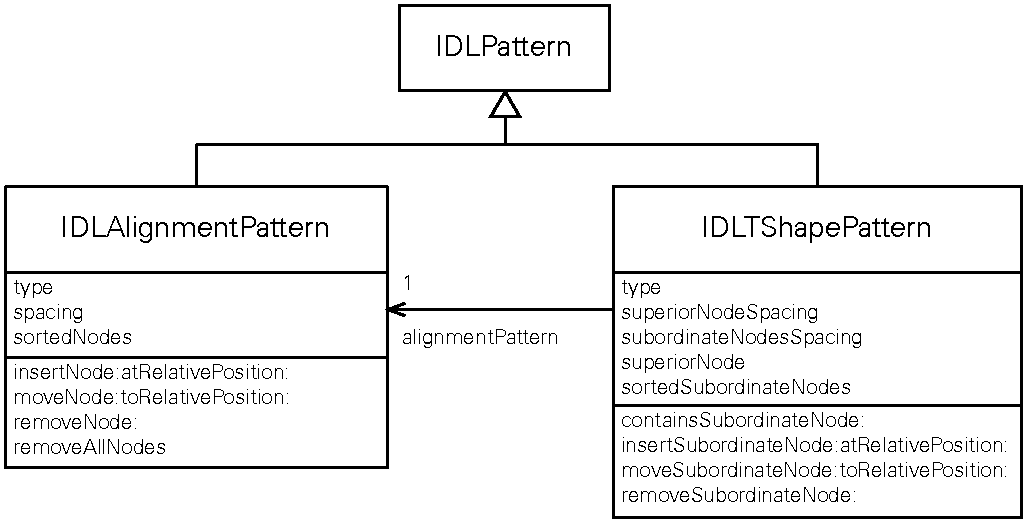
\includegraphics[width=\textwidth]{resources/layout-patterns-implementation}
    \caption{}
    \label{fig:layout-patterns-implementation}
\end{figure}

\subsubsection{Events}

\subsubsection{Engine}

% IDLLayoutEngine & Subclasses (bzw. unterstützte Layout-Engines)

% IDLLayoutEngine besitzt intern Referenzen auf den Inhalt des Diagramms und muss daher mit dem Diagramm synchronisiert werden (manuell) mit s.g. Layout-Events

% Löschen eines (oder mehreren Elementen) im Prototypen nicht unterstützt, nur hinzufügen und "rausfahren"

\subsection{Canvas View}

% Animation der Layout-Übergängen
% - implizite Core Animation Animation
% - Überführen von mehreren Animationen mit POP => wichtiger in Multi-Touch-Umgebung, bei Desktop nur ein Mauszeiger, keine parallele Aktionen

% Vergrößerung des Fensters -> Zentrierung des Inhalts (durch die Umrechnung)

% Berechnung der Start- und Endpunkte der Kanten anhand von Eigenschaften der Knoten (siehe OmniGraffle)

\subsection{Dragging Manager}

% Drag and Drop

\subsection{Application}
